

\section{Correlation Power Analysis (CPA)}

\begin{frame}
    \frametitle{From DPA to CPA: Motivation}

    \textbf{CPA} was introduced by Brier, Clavier, and Olivier (2004) as a refinement of Differential Power Analysis. 
    
    \begin{block}{Key Difference from DPA}
        \begin{itemize}
            \item DPA: compares subset averages at a single point in time.
            \item CPA: computes the \textbf{statistical correlation} between predicted leakage
                  (based on a model) and actual power measurements.
        \end{itemize}
    \end{block}
    \vspace{2mm}
    \textbf{Advantage:} Instead of just testing “is there a measurable difference?”, CPA quantifies
    \textit{how well the model matches reality}, across the whole trace.
\end{frame}

\begin{frame}
    \frametitle{Leakage Model 1: The Hamming Weight (HW)}

    The simplest model for data-dependent power leakage assumes consumption is proportional to the number of bits set to '1' in a register or on a bus.

    \begin{block}{Definition: Hamming Weight}
        For an m-bit data word $D = \sum_{j=0}^{m-1} d_j 2^j$, its Hamming Weight is the count of its '1' bits:
        \[
            HW(D) = \sum_{j=0}^{m-1} d_j
        \]
    \end{block}

    \begin{itemize}
        \item \textbf{Key Insight:} In this model, power consumption depends on the \textbf{number of active bits}, not the integer value they represent.
        \item For example, the 8-bit values \texttt{0x01}, \texttt{0x02}, \texttt{0x40}, and \texttt{0x80} all have $HW=1$ and are predicted to leak similar amounts of power.
        \item For uniformly random m-bit data, the average Hamming Weight is $m/2$.
    \end{itemize}
\end{frame}

\begin{frame}
    \frametitle{Leakage Model 2: The Hamming Distance (HD)}
    
    The HW model has a limitation: it ignores the hardware's previous state. A more physically accurate model states that power is consumed when bits \textbf{flip state} (e.g., on a data bus).

    \begin{block}{Definition: Hamming Distance}
        The Hamming Distance between a new data word $D$ and the previous state $R$ is the number of bits that have changed:
        \[
            HD(D, R) = HW(D \oplus R)
        \]
    \end{block}

    \begin{itemize}
        \item This \textbf{transition model} is a better fit for real CMOS logic, where charging and discharging capacitors during bit flips is a major source of dynamic power consumption.
        \item The $D \oplus R$ operation isolates exactly which bits have toggled.
        \item The Hamming Weight model is a special case of the HD model where the reference state $R$ is assumed to be all zeros ($R=0$).
    \end{itemize}
\end{frame}

\begin{frame}
    \frametitle{The Linear Power Model for CPA}

    The Hamming Distance model leads to the fundamental assumption of CPA: the data-dependent portion of the power consumption is linearly related to the number of bit transitions.

    \begin{alertblock}{The Linear Power Model}
    This relationship is expressed as:
    $$ W = a \cdot HD(D,R) + b $$
    \begin{itemize}
        \item $W$: The total power measured at a specific point in time.
        \item $HD(D,R)$: The \textbf{hypothesized leakage} based on the HD model.
        \item $a$: A scaling factor connecting the HD() to the actual power.
        \item $b$: A constant offset representing static power and measurement noise.
    \end{itemize}
    \end{alertblock}
    
    The entire goal of CPA is to find a key guess that makes our hypothesized leakage $HD(D,R)$ strongly correlate with the measured power $W$.
\end{frame}



\begin{frame}
    \frametitle{Limitations of Classic DPA}
    Differential Power Analysis (DPA) distinguishes key guesses 
    by comparing \textbf{average traces across two partitions}.
    
    \begin{itemize}
        \item It only considers the \textbf{difference of means} at each time sample.
        \item It is sensitive to noise: many traces required to average out randomness.
        \item May produce misleading results (\textbf{``ghost peaks''}) when leakage does not align perfectly with the partition.
        \item Wastes information: each sample is treated independently instead of considering correlation across the whole trace.
    \end{itemize}

    \begin{block}{Consequence}
        DPA is useful, but not statistically optimal; it tests for a binary difference instead of measuring \textbf{how strongly traces align with the hypothesis}.
    \end{block}
\end{frame}


\begin{frame}
    \frametitle{Why CPA is a More Powerful Refinement}

    \textbf{Correlation Power Analysis (CPA)} addresses DPA’s shortcomings:

    \begin{itemize}
        \item Uses a \textbf{parametric model} of data-dependent leakage 
              (Hamming Weight or Hamming Distance).
        \item Instead of simply asking \textit{“are two averages different?”}, 
              CPA asks: \newline
            
                  \textit{How well does my predicted power model                 
                  correlate with the measured power trace?}
              
        \item Employs the \textbf{Pearson correlation coefficient} across all traces and all times, 
              giving a continuous score for each hypothesis.
        \item Strong signals stand out as \textbf{statistically significant correlations}, 
              reducing the chance of ghost peaks.
    \end{itemize}

    \begin{block}{Intuition}
        CPA turns DPA from a binary detector into a \textbf{statistical matching process}, 
        making better use of each collected trace.
    \end{block}
\end{frame}

\begin{frame}
    \frametitle{Typical Hardware Setup for CPA}

    CPA requires:

    \begin{itemize}
        \item A device performing cryptographic operations, accessible for power measurement.
        \item A computer that sends known but random data to the device.
        \item A power measurement setup recording traces during device operation.
    \end{itemize}

    \begin{figure}
        \centering
        % Reuse your previous DPA setup image here
        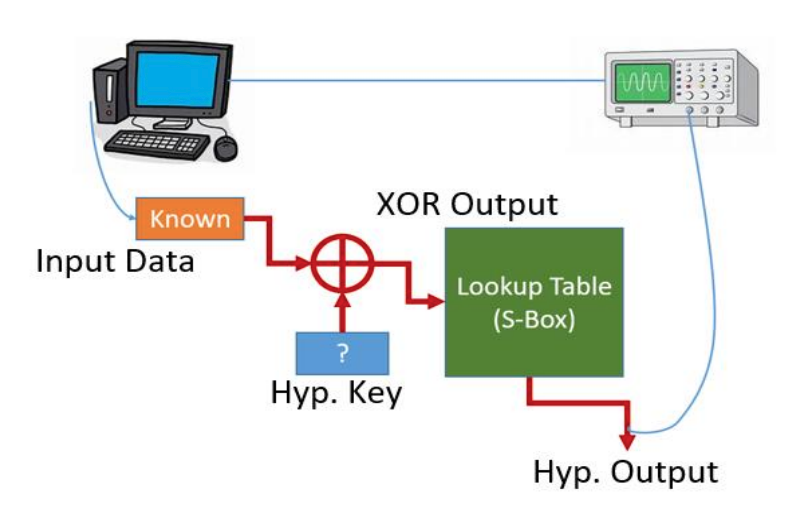
\includegraphics[width=0.7\linewidth]{main thing/Pictures/CPA_setup.png}
        \caption{Typical power measurement setup used in CPA and DPA.}
    \end{figure}
\end{frame}

\begin{frame}
    \frametitle{CPA Attack Strategy}

    The goal of a CPA attack is to find the secret key by identifying which key guess produces a \textbf{predicted power consumption} that best matches the \textbf{measured power consumption}.

    \begin{block}{The Core Question}
        For a given key guess, does the predicted Hamming Weight of an intermediate value (like the S-box output) statistically correlate with the power trace?
    \end{block}

    \begin{itemize}
        \item We perform this process for one key byte at a time.
        \item For AES-128, we target the output of the first round's \texttt{SubBytes} operation, just as we did with DPA.
        \item Intermediate value: $I_{i,n} = S[P_{i,n} \oplus K_n]$.
    \end{itemize}
\end{frame}

\begin{frame}
    \frametitle{CPA Attack on AES}

    The attack iterates through all possible values for a single key byte (e.g., $K_0$). For each guess:

    \begin{enumerate}
        \item \textbf{Hypothesize Intermediate Values:} For each trace $i=1, \dots, N$, calculate the hypothetical S-box output based on the known plaintext $P_i$ and the key guess $K_{guess}$.
        \[ V_{i, guess} = S[P_i \oplus K_{guess}] \]

        \item \textbf{Predict Leakage:} Apply the power model to each hypothetical value. For our example, we use the Hamming Weight model.
        \[ H_{i, guess} = HW(V_{i, guess}) \]
        This gives us a vector of $N$ predicted leakage values for this key guess.

        \item \textbf{Correlate:} Measure the statistical correlation between our vector of predicted leakages ($H_{guess}$) and the vector of actual power measurements at \textbf{each time sample $j$} in the traces.
    \end{enumerate}
\end{frame}

\begin{frame}
    \frametitle{The Tool for the Job: Pearson Correlation Coefficient}

    To quantify how well our predicted leakage matches the real measurements, we use the \textbf{Pearson correlation coefficient} ($\rho$).

    \begin{block}{What it Measures}
        The Pearson coefficient measures the \textbf{strength and direction of a linear relationship} between two sets of data.
    \end{block}

    Its value ranges from -1 to +1:
    \begin{itemize}
        \item $\rho = +1$: Perfect positive linear correlation.
        \item $\rho = -1$: Perfect negative linear correlation (anti-correlation).
        \item $\rho = 0$: No linear correlation.
    \end{itemize}

    \begin{alertblock}{In CPA}
    We compute $\rho$ between our hypothesized Hamming Weights and the measured power trace. A high \textbf{absolute value} of $\rho$ indicates our key guess is likely correct.
    \end{alertblock}
\end{frame}

\begin{frame}
    \frametitle{Pearson Correlation: The Definition}

    The Pearson correlation coefficient ($\rho$) is formally defined as the \textbf{covariance} of two variables, normalized by the product of their \textbf{standard deviations}.

    \begin{block}{Definitional Formula}
    \[
        \rho_{H, T_j} = \frac{\text{cov}(H, T_j)}{\sigma_H \cdot \sigma_{T_j}}
    \]
    \end{block}
    
    \begin{itemize}
        \item $\text{cov}(H, T_j)$: The covariance, which measures how our \textbf{hypothesized leakage vector ($H$)} and the \textbf{measured power vector ($T_j$)} vary together.
        \item $\sigma_H$: The standard deviation of our hypothesized leakage values
        \item $\sigma_{T_j}$: The standard deviation of the power measurements at time sample $j$ 
    \end{itemize}
    Normalizing by the standard deviations removes the units and scale, giving a pure measure of correlation between -1 and +1.
\end{frame}


\begin{frame}
    \frametitle{CPA Results: Identifying the Correct Key}

    After computing the correlation for all 256 key byte guesses at every time sample, we get 256 "correlation traces."

    \begin{itemize}
        \item The plot below shows the correlation traces for a few key candidates.
        \item The trace corresponding to the \textbf{correct key guess} will show a peak
        \item Traces for \textbf{incorrect key guesses} will fluctuate randomly around zero
    \end{itemize}

    \begin{figure}
        \centering
        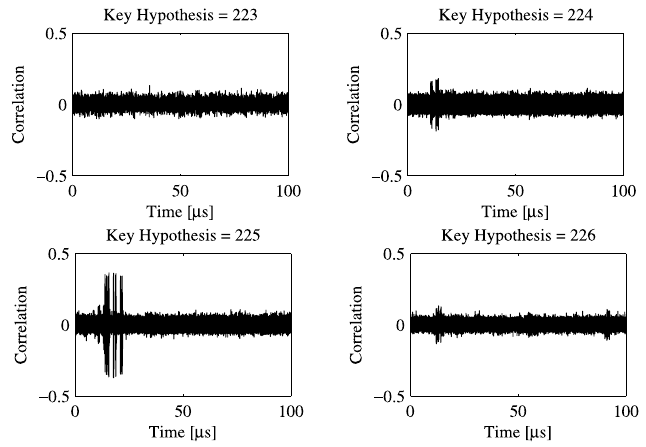
\includegraphics[width=0.7\textwidth]{main thing/Pictures/CPA_correlation_traces.png} 
        
    \end{figure}
\end{frame}

\begin{frame}
    \frametitle{Interpreting the Results: What the Peak Means}

    The peak in the correlation trace for the correct key is the "moment of truth."

    \begin{block}{The Meaning of the Peak}
        \begin{itemize}
            \item The \textbf{X-axis position} of the peak indicates the \textit{point in time} when the target intermediate value (e.g., the S-box output) is being manipulated by the device.
            \item The \textbf{Y-axis value} (the height of the peak) represents the \textit{strength} of the linear correlation ($\rho$). A higher peak means a better model fit and less measurement noise.
        \end{itemize}
    \end{block}
    For the correct key, our hypothesized leakage model, $H = HW(S[P \oplus K_{correct}])$, successfully predicts the device's actual power consumption $W$.
\end{frame}

\begin{frame}
    \frametitle{Interpreting the Results: Incorrect Guesses}
    
    When an incorrect key guess ($K_{wrong}$) is used, the predicted leakage values become meaningless.
    
    \begin{itemize}
        \item The hypothesized leakage vector, $H_{wrong} = HW(S[P \oplus K_{wrong}])$, is now a set of values that are statistically \textbf{independent} of the true intermediate value being processed inside the device.
        \item Therefore, $H_{wrong}$ is also independent of the true data-dependent power consumption, $W$.
    \end{itemize}
    
    \begin{alertblock}{The Result}
        When two data vectors are statistically independent, their Pearson correlation coefficient will naturally approach zero as the number of samples ($N$) increases. This is why the incorrect key traces appear as random noise.
    \end{alertblock}
\end{frame}
